\chapter{Vista de casos de uso}
\section{Introducción}
En esta vista nos disponemos a detallar varios casos de uso que pertenecen al sistema. Estos casos de uso son simplemente una descripción del comportamiento del sistema tal y como lo verían todos los usuarios participantes.

\section{Actores}
El sistema lo compone los siguientes usuarios:
\begin{description}
\item[Administrador] Este tipo de usuario es el encargado de crear/inicializar/eliminar los distintos entornos EHC y dispositivos.
\item[Super usuario] Este usuario es introducido en una configuración inicial por el \textit{Administrador}. El control en su entorno EHC es total, y también tiene el suficiente poder para crear distintos tipos de usuarios para los participantes del entorno EHC con unos distintos privilegios definidos por este. 
\item[Usuario] Es un tipo de usuario creado por el \textit{Super usuario}. Su funcionalidad depende de los privilegios otorgados por su creador, que puede ser desde un simple \textit{Usuario} con funciones de consulta hasta un \textit{Usuario} que pueda manipular y controlas los dispositivos del entorno EHC.
\end{description}

A través de la siguiente figura mostramos un esquema general de la organización de los actores del sistema:

\begin{center}
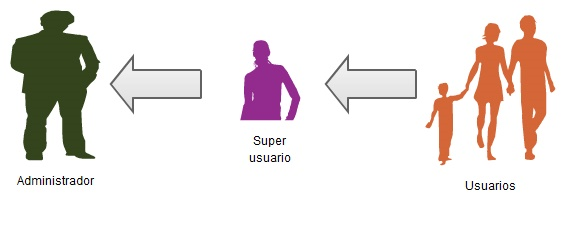
\includegraphics[width=0.7\textwidth]{4.Disenio/Imagenes/Actores}
\end{center}



\section{Casos de uso}
\subsection{Visión general de los casos de uso}
En esta sección se representan las funcionalidades y comportamientos del sistema dependiendo del tipo de usuario que se encuentre en el entorno. Gracias al estudio de los requisitos del sistema, hemos obtenido los casos de uso del sistema de una forma en la que así se agiliza el diseño del sistema y por lo tanto, su posterior implementación.
 
Mostramos a través de las figuras ~\ref{fig:cuSuperusuario} y ~\ref{fig:cuSuperusuario} los diagrama de casos de uso tanto del \textit{Super usuario} como del \textit{Administrador}. Evitamos incluir el diagrama del \textit{Usuario} ya que el \textit{Super usuario} es una extensión de este.

\begin{figure}[h!]
	\centering
	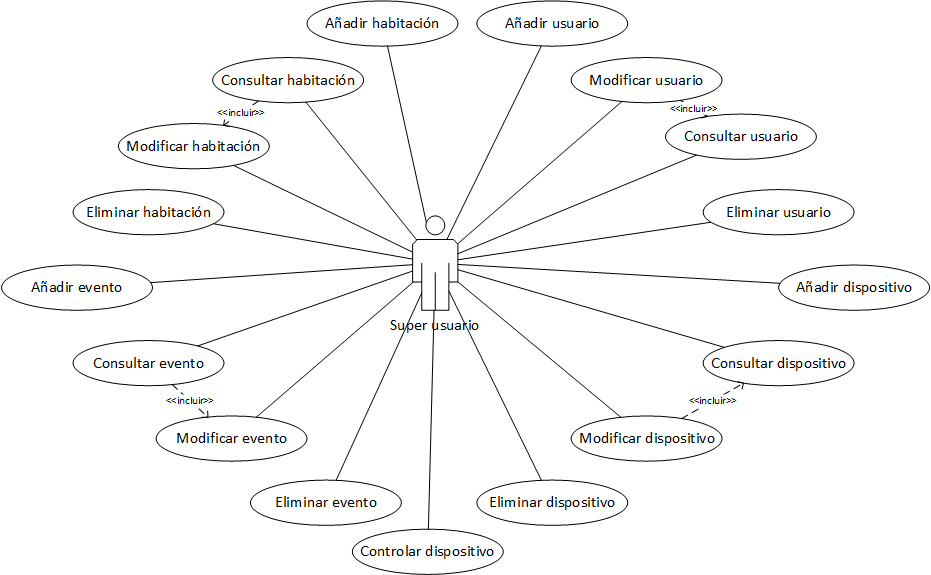
\includegraphics[width=0.7\textwidth]{4.Disenio/Imagenes/CU-Superusuario}
	\caption{Casos de uso del super usuario.}
	\label{fig:cuSuperusuario}
\end{figure}

\begin{figure}[h!]
	\centering
	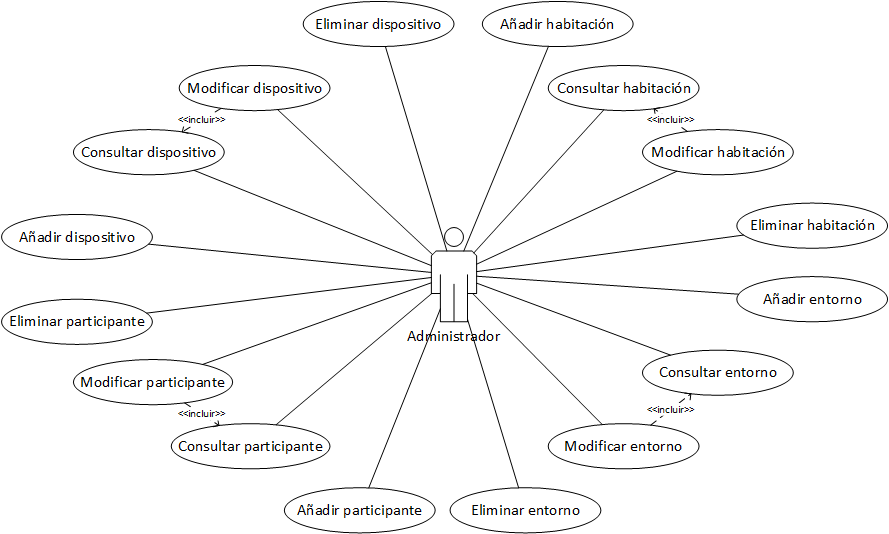
\includegraphics[width=0.7\textwidth]{4.Disenio/Imagenes/CU-Admin}
	\caption{Casos de uso del administrador.}
	\label{fig:cuAdmin}
\end{figure}


\subsection{Casos de uso en detalle}
Debido a la gran cantidad de casos de uso que hemos analizado en el sistema, la información detallada de cada uno de los casos de uso,o comúnmente conocido como \textit{Vista de escenarios}, están localizados en el documento de \textit{Casos de uso}.